% !TEX TS-program = pdfLaTeX+shellescape
% !TEX encoding = UTF-8 Unicode

\documentclass[class=beamer,tikz]{standalone}
\setbeamertemplate{navigation symbols}{} % For delete the navigation symbols
\usefonttheme{professionalfonts}
\usepackage{luatexja}
% \usepackage{pgfplots}
% \pgfplotsset{compat=1.17}

\usepackage{colortbl,array,xcolor}
\usepackage{amsmath,amsfonts}

\begin{document}
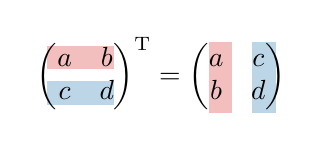
\begin{tikzpicture}
    \definecolor{tab_red}{HTML}{d62728}
    \definecolor{tab_blue}{HTML}{1f77b4}
    \definecolor{tab_green}{HTML}{2ca02c}
    %\draw[help lines] (0,0) grid (4,3);
    \path[fill=tab_red!30] (0.55,1.05) rectangle (1.40,1.35);
    \path[fill=tab_red!30] (2.60,0.50) rectangle (2.90,1.40);
    \path[fill=tab_blue!30] (0.55,0.60) rectangle (1.40,0.90);
    \path[fill=tab_blue!30] (3.15,0.50) rectangle (3.45,1.40);
    

    \node (matrix) at (2,1) {
        $\begin{pmatrix}
            a & b \cr 
            c & d
        \end{pmatrix}^{\operatorname{T}} = \begin{pmatrix}
            a & c \cr 
            b & d 
        \end{pmatrix}$
    };
\end{tikzpicture}
\end{document}